\documentclass{article}
\usepackage[margin=1in]{geometry}
\usepackage{amsmath,amsthm,amssymb}
\usepackage{bbm,enumerate,mathtools}
\usepackage{tikz,pgfplots}
\usepackage{chessboard}
\usepackage[hidelinks]{hyperref}
\usepackage{multicol} % Problem 35

\newenvironment{question}{\begin{trivlist}\item[\textbf{Question.}]}{\end{trivlist}}
\newenvironment{note}{\begin{trivlist}\item[\textbf{Note.}]}{\end{trivlist}}
\newenvironment{references}{\begin{trivlist}\item[\textbf{References.}]}{\end{trivlist}}
\newenvironment{related}{\begin{trivlist}\item[\textbf{Related.}]\end{trivlist}\begin{enumerate}}{\end{enumerate}}


\begin{document}
\rating{3}{3}
Given an $n \times n$ grid, consider all convex polygons with grid points as
vertices. Let $m(n)$ be the greatest integer $k$ such that there exists a
convex $k$-gon on the $n \times n$ grid.
\begin{figure}[!h]
  \centering
  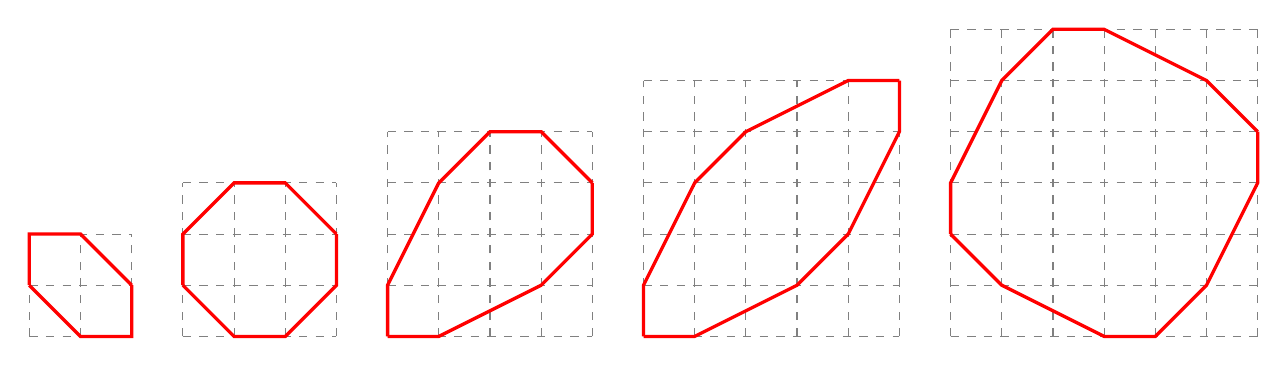
\begin{tikzpicture}[scale=0.65]
    \draw[gray, dashed] (0, 0) grid (2, 2);
    \draw[red, very thick] (0, 1) -- (1, 0) -- (2, 0) -- (2, 1);
    \draw[red, very thick] (0, 1) -- (0, 2) -- (1, 2) -- (2, 1);

    \draw[gray, dashed] (3, 0) grid (6, 3);
    \draw[red, very thick] (3, 1) -- (3, 2) -- (4, 3) -- (5, 3) -- (6,2);
    \draw[red, very thick] (3, 1) -- (4, 0) -- (5, 0) -- (6, 1) -- (6,2);

    \draw[gray, dashed] (7, 0) grid (11, 4);
    \draw[red, very thick] (7, 0) -- (7, 1) -- (8, 3) -- (9, 4) -- (10,4) -- (11,3);
    \draw[red, very thick] (7, 0) -- (8, 0) -- (10, 1) -- (11, 2) -- (11,3);

    \draw[gray, dashed] (12, 0) grid (17, 5);
    \draw[red, very thick] (12, 0) -- (12, 1) -- (13, 3) -- (14, 4) -- (16,5) -- (17,5);
    \draw[red, very thick] (12, 0) -- (13, 0) -- (15, 1) -- (16, 2) -- (17,4) -- (17,5);

    \draw[gray, dashed] (18, 0) grid (24, 6);
    \draw[red, very thick] (18, 2) -- (18, 3) -- (19, 5) -- (20, 6) -- (21,6) -- (23,5) -- (24,4);
    \draw[red, very thick] (18, 2) -- (19, 1) -- (21, 0) -- (22, 0) -- (23,1) -- (24,3) -- (24,4);
  \end{tikzpicture}
  \caption{Examples that prove $m(3) = 6, m(4) = 8, m(5) \geq 9, m(6) \geq 10,$ and $m(7) \geq(12)$}
\end{figure}

\begin{question}
  What is $m(n)$?
\end{question}

\begin{related}
  \item What is a proof (or counterexample) that the examples shown are the best possible?
  \item How does $m(n)$ grow asymptotically?
  \item Do the shapes do anything interesting in the limit?
  \item Are there finitely many maximal polygons without rotational symmetry (e.g. $m(5)$)?
  \item How does this generalize to $m \times n$ grids?
\end{related}

\begin{references}
  \item Problem 6.
  \item Problem 7.
\end{references}
\end{document}
